\chapter{Hidrostática}

\section{Ecuación fundamental de la fluidostática}

\textbf{Fluido en reposo}: No hay esfuerzos tangenciales, y la única
fuerza superficial es la presión.

Equilibrio estático: 

\begin{equation}
\vec{f}_{m}-\vec{\nabla}p=0
\end{equation}


Según el calculo diferencial, 
\[
\vec{\nabla}\times\left(\vec{\nabla}\phi\right)=0\quad\forall\phi\text{ escalar}
\]

\[
\Rightarrow\vec{\nabla}\times\vec{f_{m}}=0.
\]
 $\Rightarrow\vec{f}_{m}$ ha de ser un \emph{campo conservativo}.

\[
\dif p=\vec{f}_{m}\cdot\dif\vec{r}
\]
 Integrando sobre un determinado camino, 
\[
p\left(\vec{r}\right)=p\left(\vec{r}_{0}\right)+\int_{\vec{r}_{0}}^{\vec{r}}\vec{f}_{m}\cdot\dif\vec{r}
\]
 Nos permite calcular la presión en cualquier punto $\vec{r}$ conociendo
el valor en un punto de referencia $\vec{r}_{0}$ y el campo de fuerzas
$\vec{f}_{m}$.

Si $\vec{f}_{m}$ es conservativo 
\[
\vec{f}_{m}=-\rho\vec{\nabla}U
\]
 y, entonces, 
\[
\vec{\nabla}p=-\rho\vec{\nabla}U
\]

Si $\rho$ varia de forma arbitraria, no existen soluciones para la
ecuación , y no es posible llegar al equilibrio, $\rightarrow$ \textcolor{blue}{corrientes
convectivas}

La ecuación sólo admite soluciones cuando $\rho$ es únicamente función
de la presión, o bien es constante (fluido incompresible). 
\[
p+\rho U=cte
\]

$\rightarrow$ \textcolor{blue}{Principio de Pascal}

Hidrostática en el campo de la gravedad

\[
\vec{f}_{m}=\rho\vec{g},
\]
 con 
\[
\vec{g}=-g\vec{k}\qquad\text{donde }g=9.81\,\frac{\textrm{m}}{\textrm{s}^{2}}
\]
 y 
\[
U=gz
\]



Superficies isobáricas (superficies de igual presión), incluida la
superficie libre de los líquidos, horizontales. %

\[
\vec{\nabla}p=-\rho g\vec{k}\Rightarrow\left\{ \begin{aligned}\dparc{p}{x} & =0\\
\dparc{p}{y} & =0\\
\dparc{p}{z} & =-\rho g
\end{aligned}
\right.
\]
%

La presión es únicamente función de la coordenada $z$.

\[
\deriv{p}{z}=-\rho\,g\Rightarrow\,p_{2}-p_{1}
\]

\[
=-\int_{z_{1}}^{z_{2}}\rho\,g\,\dif z
\]
%

\subsection*{Actividad 1:}
\noindent\begin{minipage}[t]{1\columnwidth}%
\begin{itemize}
\item ¿A cuántos metros de columna de agua corresponden la presión atmosférica?
\item Si el aire fuese incompresible, con la densidad que tiene a nivel
del mar, ¿cuál debería ser la altura de la atmósfera para tener la
misma presión?
\end{itemize}
%
\end{minipage}

\section{Presión atmosférica}

La presión atmosférica disminuye con la altura. Dado que el aire es
un gas, su densidad disminuye, en general, cuando disminuye la presión,
por lo que también es menor cuando aumentamos la altura.

Necesitamos información sobre la variación de $\rho$ con $z$, o
bien con $p$.

Opción: aire gas ideal 
\[
\rho=\frac{pM}{RT}\quad\textnormal{con}\,M=28.9\,\textnormal{g/mol}.
\]
 
\begin{equation}
\Rightarrow\,\frac{\dif p}{p}=-\frac{Mg}{RT}\dif z\label{eq:general}
\end{equation}



Sin considerar la variación de $g$ con la altura: 
\begin{itemize}
\item \textcolor{blue}{Atmósfera isoterma:} 
\[
\int_{p_{0}}^{p}\frac{\dif p}{p}=-\int_{0}^{z}\frac{Mg}{RT}\dif z
\]
 
\[
\ln\frac{p}{p_{0}}=-\frac{Mg}{RT}z=-\frac{\rho_{0}g}{p_{0}}z
\]
 
\begin{equation}
\Rightarrow\boxed{p=p_{0}\exp\left(-\frac{\rho_{0}g}{p_{0}}z\right)=p_{0}\exp\left(-\frac{z}{\alpha}\right)}\label{eq:isotermica}
\end{equation}
 donde 
\[
\alpha=\frac{p_{0}}{\rho_{0}g}
\]
\end{itemize}
Valores normales: 
\[
\left.\begin{aligned}\rho_{0} & =1.292\,\text{Kg}/\text{m}^{3}\\
g & =9.80665\,\text{m}/\text{s}^{2}\\
p_{0} & =760\,\text{mmHg}=101328\,\text{Pa}
\end{aligned}
\right\} \rightarrow\alpha=7997.35\,\text{m}\approx8000\,\text{m}
\]



\begin{itemize}
\item \textcolor{blue}{Atmósfera adiabática:} 
\[
\frac{p}{\rho^{\gamma}}=\frac{p_{0}}{\rho_{0}^{\gamma}}\qquad\text{con}\qquad\gamma=\frac{c_{p}}{c_{v}}=1.4\qquad\text{para aire}
\]
\end{itemize}
\[
\dif p=-g\rho\dif z=-\rho_{0}\left(\frac{p}{p_{0}}\right)^{\frac{1}{\gamma}}g\dif z
\]
 
\[
\Rightarrow\frac{\dif p}{p^{\frac{1}{\gamma}}}=-\frac{\rho_{0}}{p_{0}^{\frac{1}{\gamma}}}g\dif z
\]

\[
\int_{p_{0}}^{p}\frac{\dif p}{p^{\frac{1}{\gamma}}}=\int_{0}^{z}-\frac{\rho_{0}}{p_{0}^{\frac{1}{\gamma}}}g\dif z=-\frac{\rho_{0}}{p_{0}^{\frac{1}{\gamma}}}gz
\]


\[
\Rightarrow\frac{1}{-\frac{1}{\gamma}+1}\left.p^{-\frac{1}{\gamma}+1}\right]_{p_{0}}^{p}=-\frac{\rho_{0}}{p_{0}^{\frac{1}{\gamma}}}gz
\]

\[
\Rightarrow\frac{\gamma}{\gamma-1}\left[p^{\frac{\gamma-1}{\gamma}}-p_{0}^{\frac{\gamma-1}{\gamma}}\right]=-\frac{\rho_{0}}{p_{0}^{\frac{1}{\gamma}}}gz
\]

\[
\Rightarrow p^{\frac{\gamma-1}{\gamma}}-p_{0}^{\frac{\gamma-1}{\gamma}}=\frac{1-\gamma}{\gamma}\frac{\rho_{0}}{p_{0}^{\frac{1}{\gamma}}}gz
\]

\begin{equation}
\Rightarrow\boxed{\left(\frac{p}{p_{0}}\right)^{\frac{\gamma-1}{\gamma}}=1+\frac{1-\gamma}{\gamma}\frac{z}{\alpha}}\label{eq:adiabatica}
\end{equation}


\begin{itemize}
\item \textcolor{blue}{Atmósfera estándar:}
\end{itemize}
En realidad, la temperatura media de la atmósfera disminuye de forma
casi lineal con la altura 
\[
T=T_{0}-Bz
\]
 hasta una altura aproximada de 11000 metros (región conocida como
\textit{troposfera}). Los valores de $T_{0}$ (la temperatura a nivel
del mar) y $B$ (\textit{gradiente térmico}) varían no sólo según
el día sino también a lo largo del mismo día. Los valores estándar
usados por convenio son 
\begin{eqnarray*}
T_{0} & = & 15^{\circ}C=288.16\textnormal{K}\\
B & = & 0.0065\textnormal{K/m}
\end{eqnarray*}



\subsection*{Actividad 2:}
Integrar la ecuación (\ref{eq:general}) con esta distribución de
temperatura para obtener 
\begin{equation}
p=p_{0}\left(1-\frac{Bz}{T_{0}}\right)^{\frac{Mg}{RB}}
\end{equation}

El valor del exponente para aire es 
\[
\frac{Mg}{RB}=5.26
\]

Después de la troposfera, la temperatura se mantiene constante hasta
unos 20000 metros para empezar a aumentar de forma gradual.

Hay que tener siempre en cuenta que esta atmósfera estándar es un
valor promediado. 

\section{Fuerza de un fluido estático sobre una superficie}

\subsection{Cálculo de la fuerza}


\begin{center}
\resizebox{0.8\textwidth}{!}{\input{TeX_files/chapter02-Hidrostatica/superficie.pdftex_t}}
\par\end{center}


\[
F=\int_{S}\dif F=\int_{S}(p_{0}+\rho\,g\,h)\dif S==\int_{S}(p_{0}+\rho\,g\,y\,\sin\theta)\dif S
\]

\[
\Rightarrow\;F=p_{0}\,S+\rho\,g\,\sin\theta\int_{S}y\dif S
\]

\begin{description}
\item [{$\int_{S}y\dif S$}] : momento de primer orden de la superficie
$S$ respecto el eje $x$ $\rightarrow$ coordenada $y_{C}$ del centroide
$C$ de la forma
\end{description}
\[
y_{C}\,S=\int_{S}y\dif S\,\Rightarrow\;F=(p_{0}+\rho\,g\,y_{C}\,\sin\theta)S=(p_{0}+\rho\,g\,h_{C})S
\]

\fbox{%
\noindent\parbox[c]{1\textwidth}{%
 La fuerza ejercida sobre una superficie totalmente sumergida se puede
calcular \textbf{imaginando} que la presión que actúa es constante
en toda la superficie e igual al valor en el centroide. %
}}


\subsection{Coordenadas del punto de aplicación}


Momento de la fuerza $\vec{F}$ respecto el eje $x$: 
\[
y_{cp}F=\int_{S}y\dif F=\int_{S}y(p_{0}+\rho\,g\,y\,\sin\theta)\dif S=p_{0}\int_{S}y\dif S+\rho\,g\,\sin\theta\int_{S}y^{2}\dif S
\]
 
\[
\Rightarrow y_{cp}F=\int_{S}y\dif F=p_{0}\,y_{C}\,S+\rho\,g\,\sin\theta I_{xx}
\]
 donde $I_{xx}$ es el momento de segundo orden de la superficie $S$
respecto el eje $x$.

Nuevo sistema de coordenadas $(\xi,\eta,\zeta)$, paralelo a $(x,y,z)$
pero con origen en el centroide $C$. 
\[
I_{xx}=I_{\xi\xi}+y_{C}^{2}\,S\qquad\text{(T. de Steiner)}
\]

\[
\Rightarrow y_{cp}=y_{C}+\frac{I_{\xi\xi}}{\left(y_{C}+\frac{p_{0}}{\rho\,g\,\sin\theta}\right)S}
\]


Para $x_{cp}$: 
\[
\int_{S}x\dif F=\int_{S}x(p_{0}+\rho\,g\,y\,\sin\theta)\dif S=p_{0}\int_{S}x\dif S+\rho\,g\,\sin\theta\int_{S}xy\dif S
\]
 
\[
\Rightarrow\int_{S}x\dif F=p_{0}\,x_{C}\,S+\rho\,g\,\sin\theta I_{xy}
\]
 
\[
I_{xy}=I_{\xi\eta}+x_{C}\,y_{C}\,S\qquad\text{(T. de Steiner)}
\]
 
\[
\Rightarrow x_{cp}=x_{C}+\frac{I_{\xi\eta}}{\left(y_{C}+\frac{p_{0}}{\rho\,g\,\sin\theta}\right)S}
\]



Normalmente, $p_{0}$ (en general, la presión atmosférica) actúa por
igual en las dos caras de la superficie, 
\begin{align*}
F & =\rho\,g\,h_{C}\,S\\
x_{cp} & =x_{C}+\frac{I_{\xi\eta}}{y_{C}\,S}\\
y_{cp} & =y_{C}+\frac{I_{\xi\xi}}{y_{C}\,S}
\end{align*}

Dado que $I_{\xi\xi}$ es, por definición, una cantidad siempre positiva,
el centro de presiones se encuentra siempre por debajo del centroide.


\subsection{Fuerza sobre una superficie curva totalmente sumergida}


\begin{center}
\resizebox{!}{5cm}{\input{TeX_files/chapter02-Hidrostatica/superficie_curva.pdftex_t}}
\par\end{center}

 
\[
\begin{aligned}F_{x} & =-\int_{S}(p_{0}+\rho\,g\,h)\dif S_{x}\\
F_{y} & =-\int_{S}(p_{0}+\rho\,g\,h)\dif S_{y}
\end{aligned}
\]
 

Si proyectamos la superficie $S$ sobre los planos $x=0$ y $y=0$,
obtenemos $S_{x}$ y $S_{y}$, y podemos calcular $F_{x}$ y $F_{y}$,
así como sus puntos de aplicación.

$F_{z}$ resulta ser igual al peso total de fluido que se encuentra
\emph{por encima} de la superficie curva. La linea de acción de $F_{z}$
pasa por el centro de gravedad de la columna de fluido que hay sobre
la superficie.

Las expresiones anteriores son válidas únicamente para fluidos con
densidad constante. Si el fluido está estratificado, de forma que
hay un \textit{gradiente de densidad}, positivo hacia la dirección
vertical negativa, los cálculos se complican.


\subsection*{Actividad 3:}
Calcula la fuerza, y su punto de aplicación, que hace un embalse de agua de 50
metros de profundidad y 200 metros de ancho sobre la pared, vertical,
de la presa.


\section{Principio de Arquímedes}

\fbox{%
	\parbox{1\textwidth}{%
%\begin{quotation}
	\emph{Todo cuerpo sumergido, completa o parcialmente,
		en un fluido experimenta
		un empuje dirigido verticalmente hacia arriba, con magnitud igual al peso del
		fluido desalojado y cuya  linea de acción pasa por el centro de gravedad
		del fluido desalojado}
%\end{quotation} %
}}


\begin{minipage}{0.4\textwidth}
	\begin{center}
		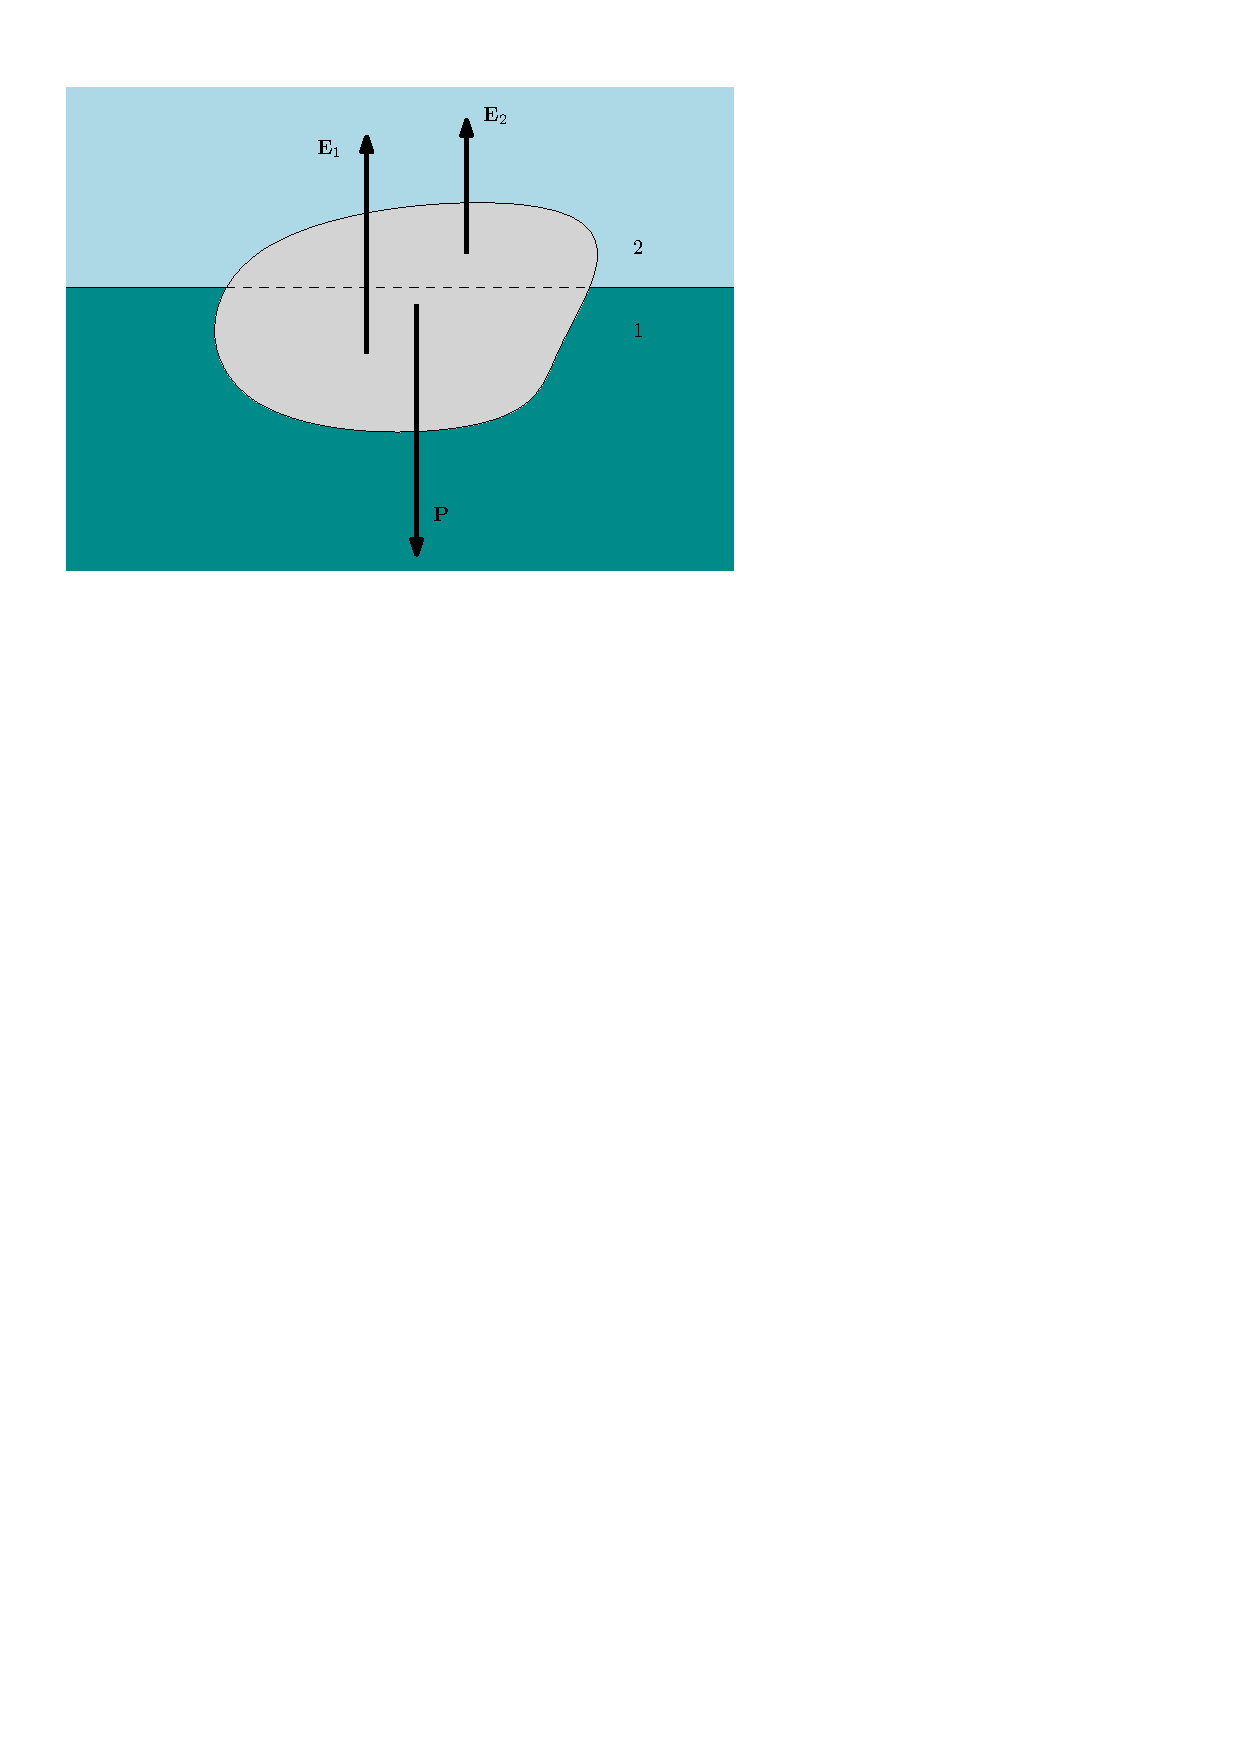
\includegraphics[width=\textwidth]{TeX_files/chapter02-Hidrostatica/arquimedes}
	\end{center}
\end{minipage}
\begin{minipage}{0.5\textwidth}
	Las lineas de acción de las fuerzas de empuje y el peso no
	tienen porqué coincidir, y, en este caso, se producen pares de fuerzas.
	\begin{description}
		\item[\textcolor{blue}{carena}] volumen del fluido desalojado
		\item[\textcolor{blue}{centro
			de carena} o \textcolor{blue}{centro de empuje}] centro de gravedad del fluido desalojado
	\end{description}
\end{minipage}


	El principio de Arquímedes no es, en realidad, un principio. Se puede deducir en cualquier caso simplemente calculando la integral de la presión sobre la superficie que limita el cuerpo.
	
	También se puede obervar que es la resta del peso de la columna de fluido sobre la superficie superior y sobre la superficie inferior.
	
\begin{center}
	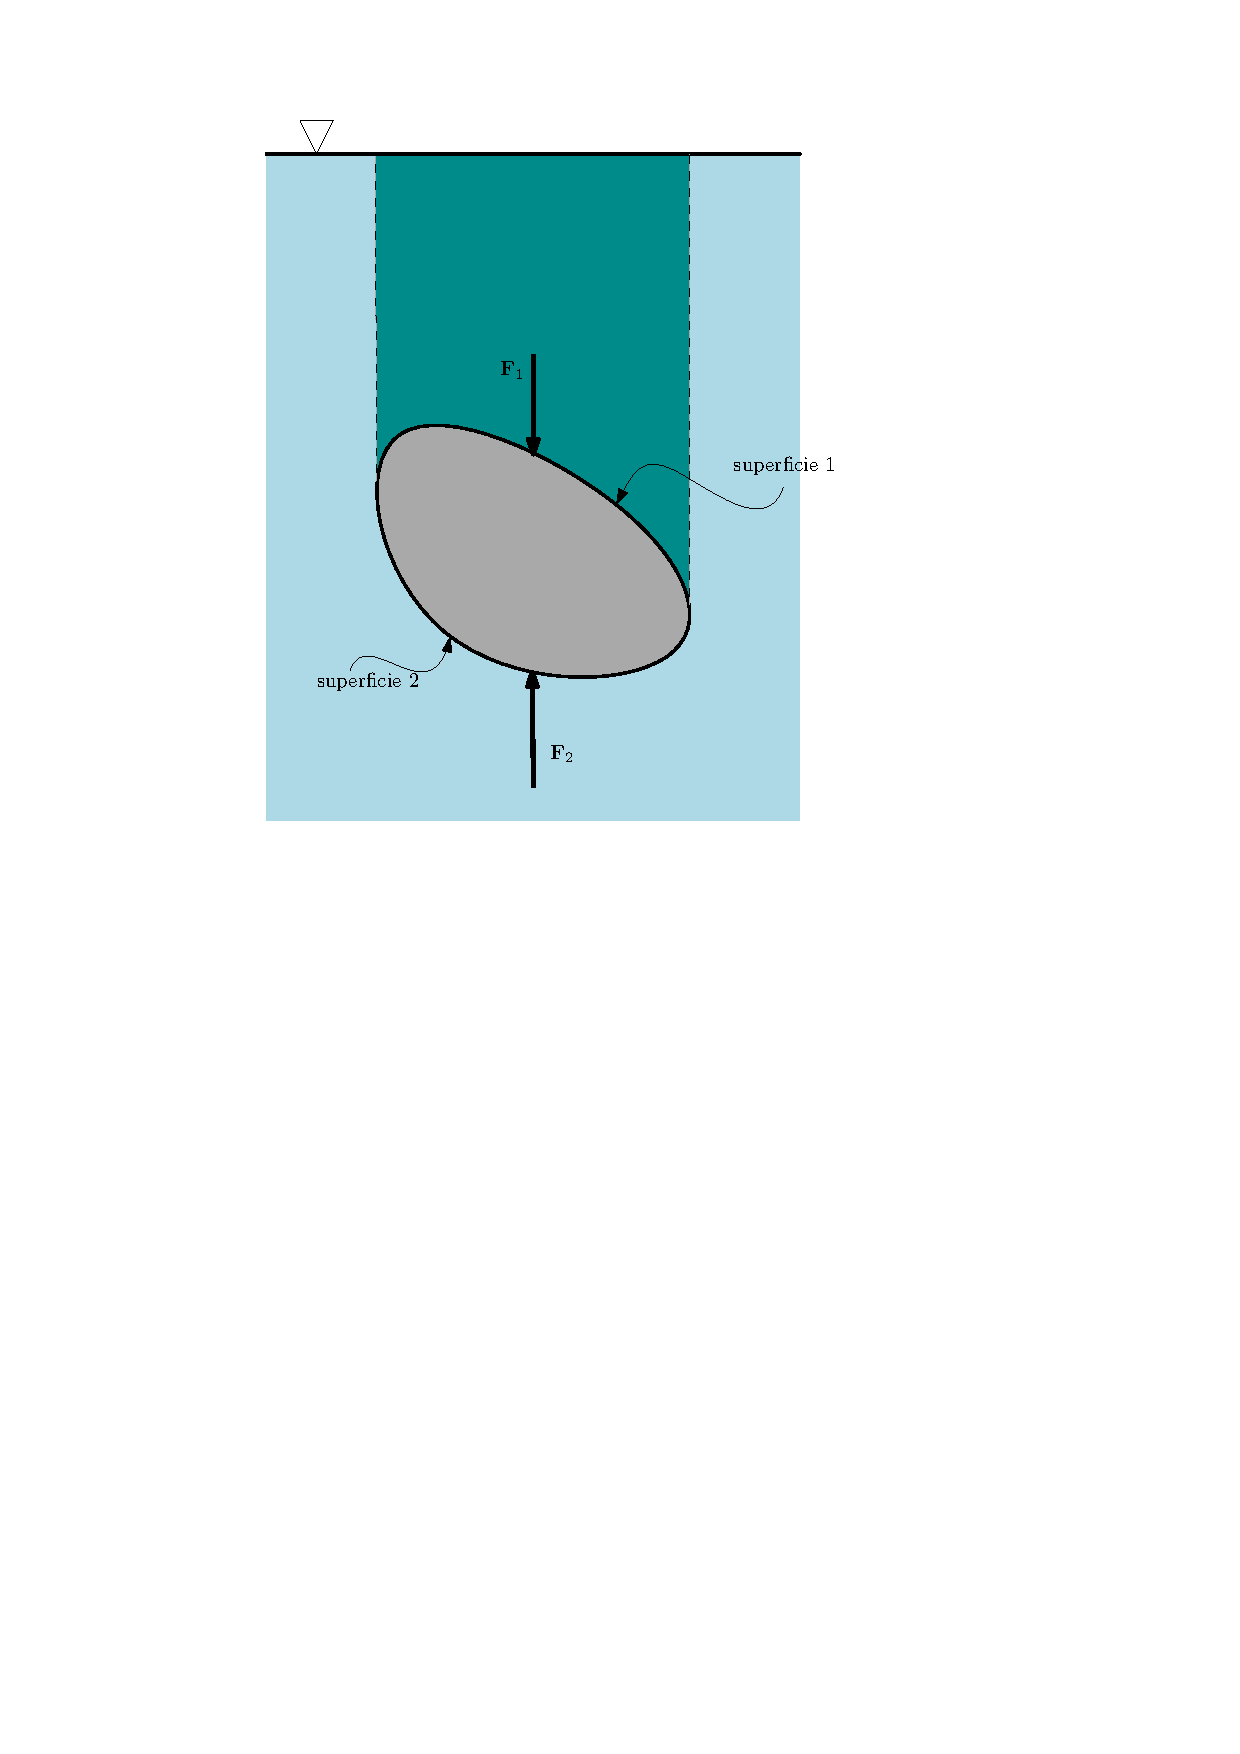
\includegraphics[width=0.5\columnwidth]{TeX_files/chapter02-Hidrostatica/arquimedes2}
\end{center}
\section{Segunda ley de Arquímedes}


	La segunda ley de Arquímedes dice que \emph{un cuerpo que flota desaloja su propio peso de fluido}. 
	
	Se puede comprender observando que en la figura, el recipiente con solo fluido y el que tiene fluido y cuerpo flotando, \textbf{deben pesar lo mismo}. Pregunta: ?`Cómo sabemos que pesan lo mismo?


	\begin{center}
		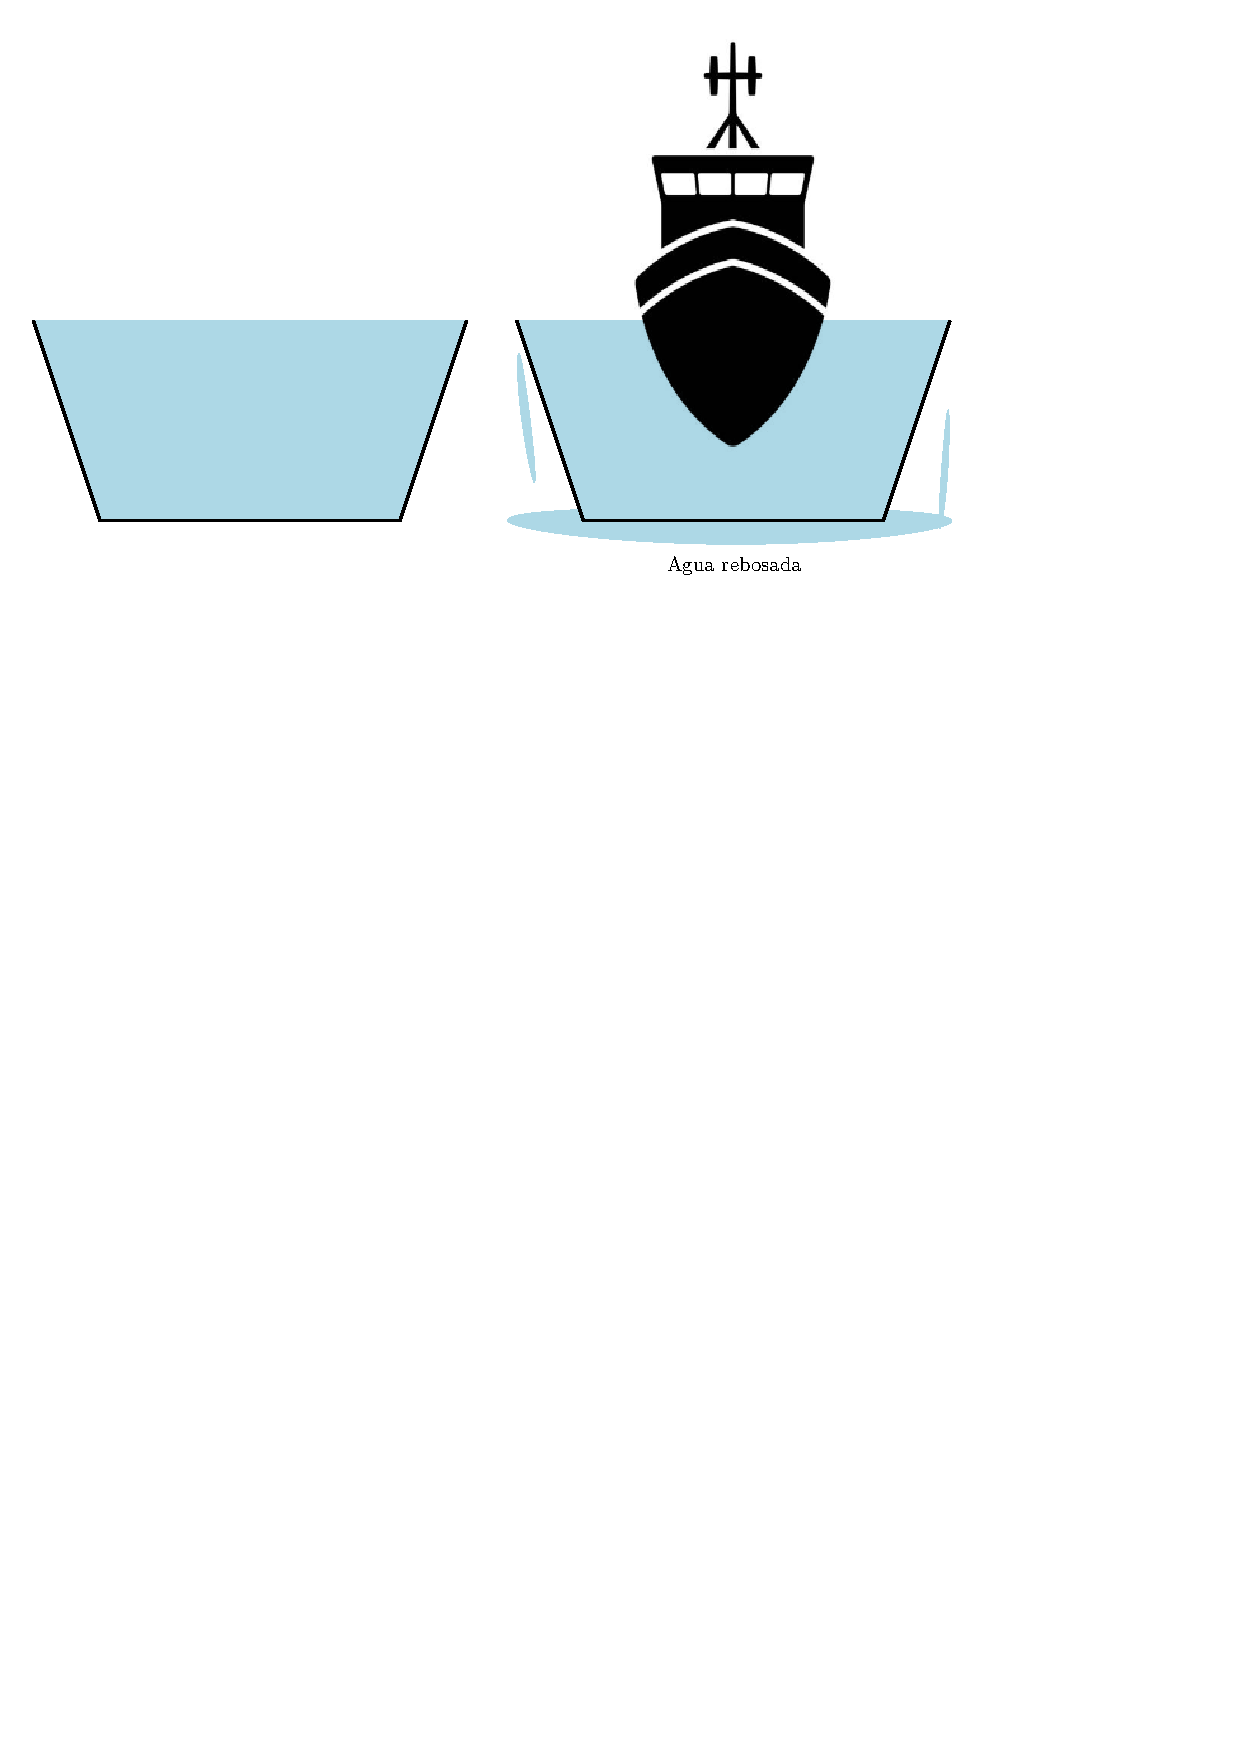
\includegraphics[width=0.75\columnwidth]{TeX_files/chapter02-Hidrostatica/arquimedes1}
	\end{center}


\section{Estabilidad}

Para un cuerpo sumergido, el centro de gravedad puede ser diferente del centro de empuje, y esto produce un momento que puede ser restaurador (equilibrio estable) o de vuelco (equilibrio inestable)

\begin{center}
	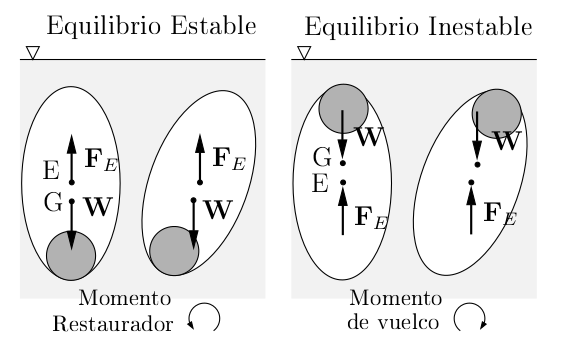
\includegraphics[width=0.7\linewidth]{TeX_files/chapter02-Hidrostatica/estabilidad1}
\end{center}

%\begin{center}
%	\includegraphics[width=0.7\columnwidth]{estab1.png}
%	% estab1.png: 996x491 pixel, 72dpi, 35.14x17.32 cm, bb=
%\end{center}


Para un cuerpo flotante, es más complicado, ya que la posición del centro de empuje varía


Equilibrio estable 
\begin{center}
	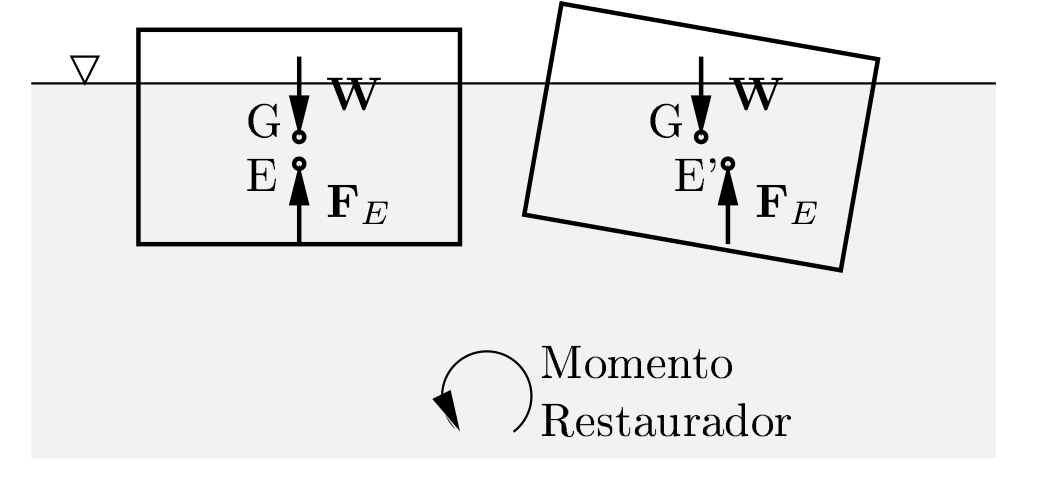
\includegraphics[width=0.7\linewidth]{TeX_files/chapter02-Hidrostatica/estabilidad2}
\end{center}



Equilibrio inestable
\begin{center}
	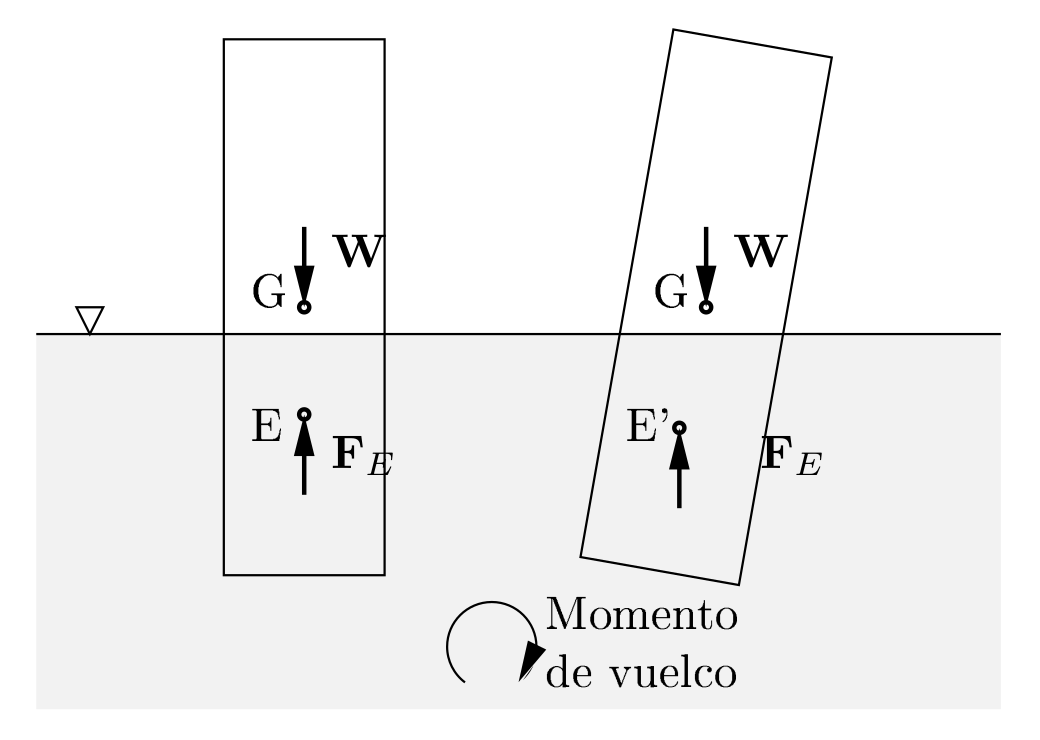
\includegraphics[width=0.7\linewidth]{TeX_files/chapter02-Hidrostatica/estabilidad3}
\end{center}


Pasos para calcular la estabilidad de un cuerpo flotante, consideremos un cuerpo simétrico:

1.- Se calcula posición de equilibrio inicial, mediante las fuerzas $\vec F_E$ y $\vec W$, y sus puntos de aplicación, $E$ y $G$. Como el cuerpo estan en equilibrio, estas fuerza se alinean con el eje de simetria.

2.- Se realiza una peque\~na perturbación $\Delta \theta$. El centro de empuje se desplaza a una nueva posición $E'$. La vertical sobre $E'$ corta el eje de simetria en un punto $M$, denominado \textbf{metacentro}. Si el ángulo $\Delta \theta$ es peque\~no, el metacentro no dependerá de él.

3.- Se calcula la \textbf{altura metacéntrica}, que es la distancia de $M$ a $G$. Si $M$ está por encima de $G$, la altura metacéntrica  es positiva, y la posición es \emph{estable}. Si está por debajo, la altura metacéntrica es negativa, y la posición es \emph{inestable}.

La altua metacéntrica es una característica de la sección transversal del cuerpo y su distribución de masa.

\begin{center}
	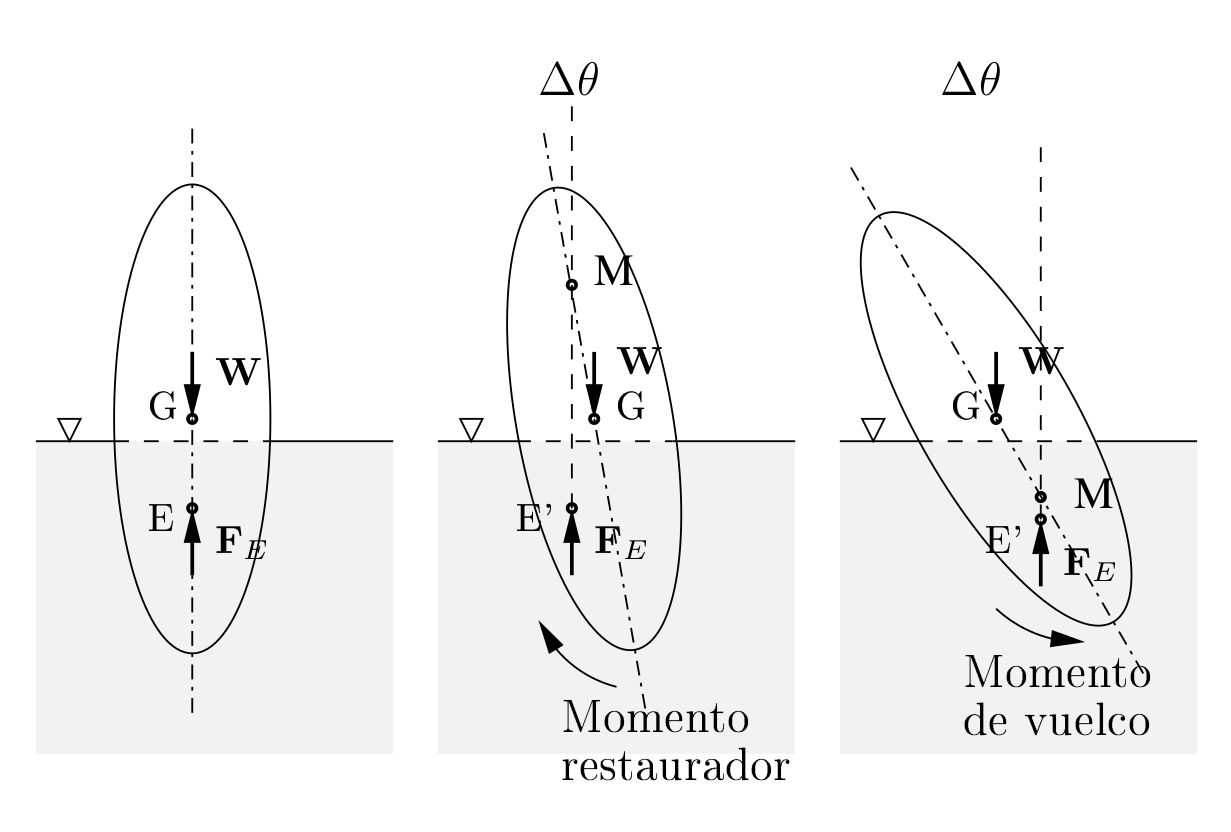
\includegraphics[width=0.7\linewidth]{TeX_files/chapter02-Hidrostatica/estabilidad4}
\end{center}

\begin{center}
	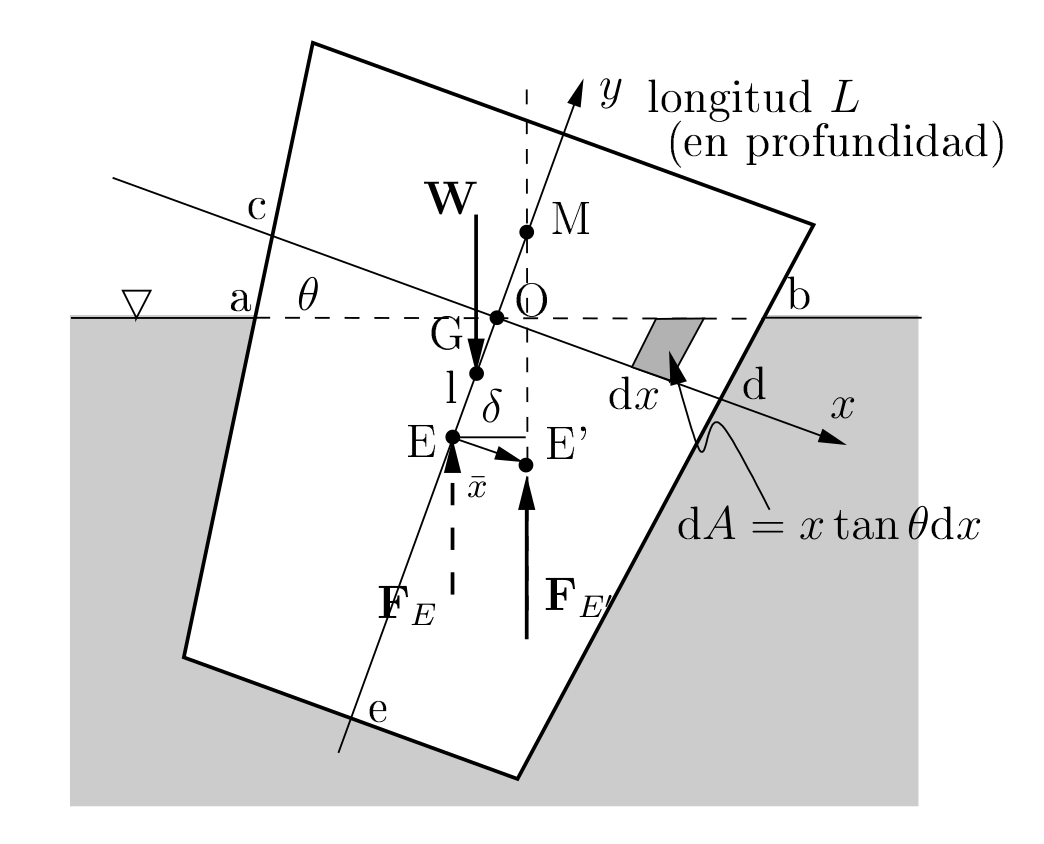
\includegraphics[width=0.7\linewidth]{TeX_files/chapter02-Hidrostatica/estabilidad5}
\end{center}




	La posición del nuevo centro de empuje se calcula con la estimación del centro de masas:

\begin{align*}
	\overline{x}V_{aObdea} &= \int_{Obd}x \dif V - \int_{cOa} x \dif V
\\
	&= \int_{Obd} x L \dif A - \int_{cOa} x L \dif A 
\\
	&= \int_{Obd} x L (x\tan \theta \dif x) - \int_{cOa} x L  (-x\tan \theta \dif x)
\\
	&= \tan \theta \int x^2 2 L \dif x = \tan \theta \int x^2 \dif A 
	\\
	&= \tan \theta I_0
\end{align*}


La altura metacéntrica es

\begin{equation}
	\overline{MG} = \overline{ME}-\overline{GE}= \frac{\overline{x}}{\tan \theta} - \overline{GE} 
= \frac{I_0}{V_{\textrm{sumergido}}} - \overline{GE} = \frac{\rho g I_0}{W} - \overline{GE}
\end{equation}

Si $\overline{MG}$ es positiva, el equilibrio es estable (para peque\~nas perturbaciones). Si 
$\overline{GE}$ es negativa, el equilibrio es estable siempre

\section[Presiones con aceleración]{Distribución de presiones en movimiento acelerado de Fluido como sólido rígido}

\subsection{Introducción. Equilibrio de una partícula}

En el caso general de un fluido que se mueve con una aceleración $\vec{a}$, la ecuación de la dinámica, bajo una distribución de presiones y la gravedad es
\begin{equation}
	\rho \vec a = -\vec \nabla p+ \rho \vec g,
\end{equation} 
suponiendo que no existen movimientos relativos entre las moléculas del fluido, de forma no existen esfuerzos tangenciales. Es decir, que el fluido se mueve en su totalidad como un \textbf{sólido rígido}.

En estas condiciones, la distribución de presiones se puede obtener con 
\begin{equation}
	\vec \nabla p = \rho (\vec g-\vec a)
	\label{ec:principal}
\end{equation} 


El movimiento más general de una partícula es una combinación de traslación más rotación respecto de un cierto punto $O$
\begin{equation}
	\vec v = \vec v_0 + \vec \Omega \times \vec v_0
\end{equation} 

\begin{equation}
	\Rightarrow \vec a = \underbrace{\deriv{\vec v_0}{t}}_{\textrm{ac. lineal}} + \underbrace{\vec \Omega \times \left( \vec \Omega \times \vec r_0\right)}_{\textrm{ac. centrípeta}} + \underbrace{\deriv{\vec \Omega}{t} \times \vec r_0}_{\textrm{ac. rotacional}}
	\label{ec:SR}
\end{equation} 

\begin{center}
	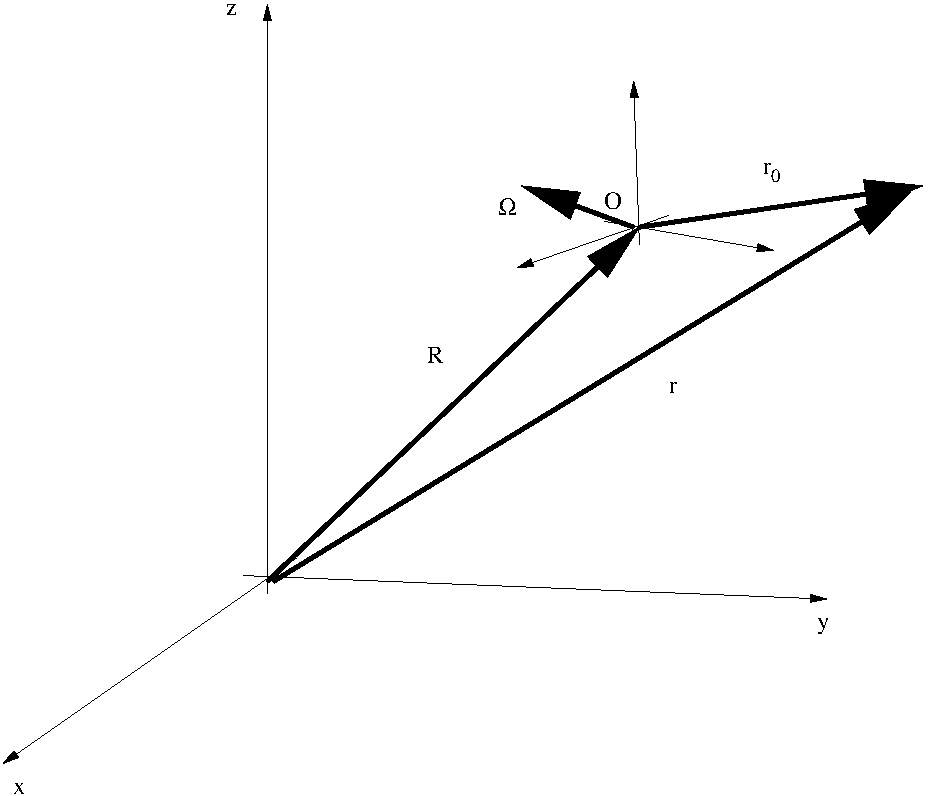
\includegraphics[width=0.7\linewidth]{TeX_files/chapter02-Hidrostatica/sistema}
\end{center}


\subsection{Aceleración lineal}

Supongamos que la aceleración se encuentra en el plano $yz$. La ecuación \ref{ec:principal} es un sistema de dos ecuaciones, una para cada dirección:
\begin{eqnarray}
	\dparc{p}{x} &=& -\rho a_x \\
	\dparc{p}{z} &=& -\rho g - \rho a_z
\end{eqnarray} 

\begin{center}
	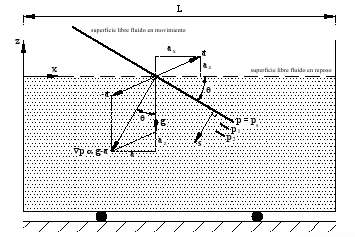
\includegraphics[width=0.7\columnwidth]{TeX_files/chapter02-Hidrostatica/ac_lineal1}
	% ac_lineal1.png: 355x237 pixel, 72dpi, 12.52x8.36 cm, bb=0 0 355 237
\end{center}

La primera ecuación da
\begin{equation}
	p = -\rho a_x x + f(z)
\end{equation} 
Derivando respecto de $z$ e igualando con la segunda ecuación obtenemos
\begin{equation}
	f'(z) = -\rho g - \rho a_z
\end{equation}
que, al integrarla, da
\begin{equation}
	f(z) = -\rho(g+a_z)z + C,
\end{equation}  
de forma que 
\begin{equation}
	\boxed{ p = -\rho a_x x -\rho(g+a_z)z + C}
\end{equation} 

\subsection*{Actividad 4:} ?`Cuánto vale la pendiente de las lineas de presión constante?

\subsection*{Actividad 5:} Si un fluido tiene tan sólo aceleración vertical, ?`cómo es la distribución de presiones? Si un depósito de 1 m de altura cae en caida libre, ?`cuál es la presión en el fondo del mismo?

\subsection{Rotación como sólido rígido}

Supongamos ahora un recipiente cilíndrico, de radio $R$, con un fluido hasta una altyua $h$, que gira con velocidad angular $\vec \Omega = \Omega \vec k$ constante. Al cabo de un cierto tiempo, todo el fluido se moverá como un sólido rígido.

\begin{center}
	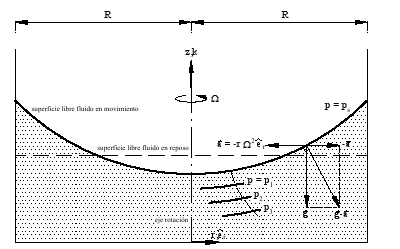
\includegraphics[width=0.7\columnwidth]{TeX_files/chapter02-Hidrostatica/ac_centripeta}
	% ac_centripeta.png: 400x249 pixel, 72dpi, 14.11x8.78 cm, bb=
\end{center}

Usando la ecuación \ref{ec:SR}, con $\deriv{\vec v_0}{t} = \deriv{\vec \Omega}{t} \times \vec r_0 =0$, tenemos tan sólo la aceleración centrípeta
\begin{equation}
	\vec \Omega \times \left( \vec \Omega \times \vec r_0\right) = -r\Omega^2 \vec e_r
\end{equation} 


Ahora hay que recordar cómo es el gradiente en coordenadas cilíndricas,
\begin{equation}
	\vec \nabla p = \dparc{p}{r} \vec e_r + \frac{1}{r}\dparc{p}{\theta}\vec e_\theta + \dparc{p}{z}\vec k,
\end{equation} 
de forma que la ecuación \ref{ec:principal} queda como
\begin{eqnarray}
	\dparc{p}{r} &=& \rho r\Omega^2 \\
	\dparc{p}{z} &=& -\rho g
\end{eqnarray} 

Actuando de la misma forma que con aceleración lineal, llegamos a la expresión
\begin{equation}
	p = \frac{1}{2}\rho \Omega^2 r^2 - \rho g z + C 
\end{equation} 


El valor de $C$ no es ni más ni menos que el valor de la presión en el origen de coordenadas, $p_0$.
\begin{equation}
	p = \frac{1}{2}\rho \Omega^2 r^2 - \rho g z + p_0 
	\label{ec:rot1}
\end{equation} 

La superficie libre se encuentra, como en el caso de la aceleración lineal, mediante conservación del volumen total del fluido (suponiendo, claro, que no se derrame). 

Sea $h_0$ la altura de la superficie libre en $(x,z)=(0,0)$. La presión en este punto es entonces $p_0=p_a + \rho g h_0$, donde $p_a$ es la presión ambiente en el exterior del líquido. La ecuación \ref{ec:rot1} queda entonces como 
\begin{equation}
	p = \frac{1}{2}\rho \Omega^2 r^2 - \rho g z + p_a + \rho g h_0
	\label{ec:rot2}
\end{equation} 
y la forma de la superficie libre, $z=z_s$, viene dada por los puntos en los que $p=p_a$. Es decir,
\begin{equation}
	\frac{1}{2}\rho \Omega^2 r^2 - \rho g z_s + \rho g h_0 = 0
\end{equation} 
\begin{equation}
	\Rightarrow  z_s = h_0 + \frac{1}{2}\frac{\Omega^2 r^2}{g} 
\end{equation} 

Para calcular $h_0$, consideramos que el volumen se conserva,

\begin{minipage}{0.5\columnwidth}
	\begin{center}
		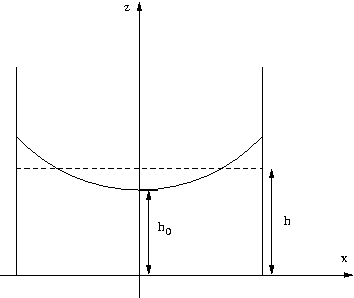
\includegraphics[width=\columnwidth]{TeX_files/chapter02-Hidrostatica/rotando}
		% rotando.png: 354x298 pixel, 80dpi, 11.24x9.46 cm, bb=0 0 319 268
	\end{center}
\end{minipage}
\begin{minipage}{0.5\columnwidth}
	\[
	\pi R^2 h = \int_0^R 2\pi r z_s \dif r =
	\]
	\[
	= \int_0^R 2\pi r\left(h_0 + \frac{1}{2}\rho\frac{\Omega^2r^2}{g}\right) \dif r =
	\]
	\[
	= \pi\left[R^2 h_0 + \frac{1}{4}\frac{\Omega^2 R^4}{g} \right]
	\]
	\[
	\Rightarrow \quad h_0 = h-\frac{1}{4}\frac{\Omega^2 R^2}{g}
	\]
	\[
	\Rightarrow z_s(r) = h-\frac{1}{4}\frac{\Omega^2 R^2}{g} + \frac{1}{2}\frac{\Omega^2 r^2}{g}
	\]
	
\end{minipage}